\chapter{分析方法}
\section{问题定义}
\label {define_problem}
第一章中对本文所要解决的问题进行了简要介绍。下面对该问题进行正式的定义。

\begin{problem}
	\label {origin}
	针对某软件系统s,假设已有版本$v_1$和$v_2$,其中补丁$p_1$是针对版本$v_1$而设计,应用后能使其演进到版本$v_3$,问$p_1$是否能够应用于版本$v_{2}$,并且应用之后是否会发生冲突?
\end{problem}

考虑到补丁间不兼容的实质是因为在应用时和应用后出现了错误,可以具体将错误分为两类:

\begin{definition}
	兼容性错误——将补丁$p_i$和补丁$p_j$先后应用于同一版本代码$v_k$时和之后所出现的程序错误。主要分为两类:
	\begin{itemize}
		\item 语法错误:即在应用一补丁$p_i$之后,再次应用另一补丁$p_j$时出现语法结构上的错误。易由编译器发现。
		\item 语义错误:将补丁$p_i$中的变更和补丁$p_j$中的变更应用于源代码之后,由于语义上的变更互相冲突而导致出现了功能上的错误,较难发现。
	\end{itemize}
\end{definition}

可以发现,该问题的核心包括两点,即:
\begin{itemize}
	\item 如何将一个专为版本$v_1$设计的补丁$p_1$成功应用于版本$v_2$上。即如何消去补丁应用过程中的语法错误。
	\item 如何检测补丁在应用于新版本之后是否会与该版本代码产生冲突?即如何检测补丁应用之后的语义错误。
\end{itemize}

下面分别对这两点进行分析和阐述。

\subsection{补丁应用}

实际上,补丁程序是专门为某一版本的软件系统所设计,因而往往不能直接应用到其他版本的代码上,而且强行应用往往会出现很多错误。常见的问题可能包括:

\begin{enumerate}
	\item 补丁程序中所提及的行不在原位置。
	\item 补丁程序中所要删除的行其实已被删除,或者所要添加的行其实已被添加。
	\item 补丁程序中所提及的文件未找到。
\end{enumerate}

由于有这些可能的问题存在,导致我们无法直接将补丁程序应用到其他版本的补丁上。因此,我们可以考虑去解决这样一个子问题。

\begin{problem}
	\label {patch_reversion}
	由于补丁p针对版本$v_{1}$设计,当尝试将其应用到版本$v_{2}$上时,可能会出现程序语法结构上的错误。如何将p成功应用到版本$v_{2}$上,使得该过程不会出现引入程序语法错误?
\end{problem}

为了更清楚的描述该问题,我们可以将其进一步形式化定义如下:

\begin{definition}
	$Code$——指源代码。
\end{definition}

\begin{definition}
	$Patch$——指补丁。
\end{definition}

\begin{definition}
	$patch: Patch \times Code \mapsto Code$。$patch(p_i,v_k) = v_m,i,k,m \subset \mathbb{N}$。该函数用于表示补丁应用的过程。
\end{definition}

\begin{definition}
	$compile: Code \mapsto Boolean$。compile函数用于表示对源代码的编译过程,如果成功编译则表示源代码中没有语法错误。
\end{definition}

\begin{definition}
	$design: Patch \times Code \mapsto Boolean$。该函数用于表示某个补丁是否为某个版本的代码而设计。
\end{definition}

\begin{problem}
	\label {app_formal}
	给定$p_i$,$v_k$,问$design(p_i,v_k) == False$时,能否使得$compile(patch(p_i,v_k)) == True$?其中$p_i \subset Patch,v_k \subset Code,i,k \subset \mathbb{N}$。
\end{problem}

可见,该问题的核心在于如何给出合适的$patch(p_i,v_k)$函数。

\subsection{补丁冲突}

就如何检测补丁在应用于新版本之后是否会与该版本代码产生冲突而言,直接去寻找冲突的存在是一件让人困惑的事情,什么是冲突?为什么会发生冲突?怎么进行检测?

因此本文考虑从另一个角度来看待这个问题。

实际上,考虑到从版本$v_1$到版本$v_2$的演进过程同样可以使用补丁来完成。那么可以考虑将这个演进过程表述成为合适的变更,得到另外一个补丁。

\begin{definition}
	\label {define_diff}
	$p = diff(v_i,v_j),i,j \subset \mathbb{N}$。该函数用于求解两个不同版本的程序$v_i$和$v_j$之间的差异性,其结果即为补丁p。
\end{definition}

从问题\ref {origin}中可以发现,$p_{1} = diff(v_{1},v_{3})$。如果同样给定$p_{2} = diff(v_{1},v_{2})$,并且已经解决了问题\ref {app_formal},那么,如何检测补丁在应用于新版本之后是否会与该版本代码产生冲突这一问题就可以规约如下。

\begin{problem}
	\label {compatible}
	给定针对某同一版本代码$v_k$的补丁$p_i$和$p_j$,问分别应用于$v_k$之后,这两个补丁对于该版本代码的语义影响是否会产生冲突?
\end{problem}

这样一来,问题的实质就清楚了。显然,该问题是由于两个补丁同时对同一版本代码造成了语义影响而造成的。那么为了回答这个问题,我们需要明确的知道到底什么是补丁对代码的影响,以及什么是冲突?

本文首先讨论什么是补丁对代码的语义影响。

\begin{definition}
	语义影响(Semantic Impact)——假如某个代码结构对其他代码结构存在依赖关系,那么就说这两者间存在语义影响。其中代码结构指程序的语法结构,包括类、方法、语句等不同的类型。
\end{definition}

事实上,如果给出不同的依赖关系的定义,那么就会得到不同类型的影响。可见,这里所谓的语义影响即是程序代码间的耦合关系。常见的依赖关系包括控制依赖和数据依赖等。下面给出语义影响的形式化定义。

\begin{definition}
	$Structure \to Class \mid Method \mid Statement \mid ...$。Structure用于表示程序代码结构,可以任意替换为对应的子类型。
\end{definition}

\begin{definition}
	$Struct: Code \mapsto \{ Structure \}$。Sturct函数定义为一个从源代码到该源代码的所有代码结构集合的映射。
\end{definition}

\begin{definition}
	$im: Structure \mapsto Structure$。影响关系定义为一个从代码结构到代码结构的映射关系。
\end{definition}

\begin{definition}
	$depend: Structure \mapsto Structure$。依赖关系定义为一个从代码结构到代码结构的映射关系。
\end{definition}

\begin{definition}
	$\forall structure_i,structure_j \subset Struct(v_k),  im(structure_i) = structure_j \iff depend(structure_i) = structure_j$,其中$v_k \subset Code$。
\end{definition}


\begin{definition}
	\label {define_conflict}
	语义冲突(Confilict)——指两个补丁所对应的不同变更集合之间存在某两条互斥的变更。
	其中两条变更互斥指二者的语义互相影响。
\end{definition}

下面给出其形式化的定义。

\begin{definition}
	$Change$——指变更。$Patch = {Change}$。
\end{definition}

\begin{definition}
	$change: Structure \mapsto Change$。用于表示代码结构和其所对应的变更的映射。
\end{definition}

\begin{definition}
	$Pat: Code \mapsto \{Patch\}$。用于表示代码到其对应的补丁集合的映射。
\end{definition}

\begin{definition}
	$conflict: Patch \times Patch \mapsto Boolean$。如果$\exists im(structure_i) = structure_k \land im(structure_j) = structure_k$,其中$structure_i,structure_j,structure_k \subset v_t,change(structure_i) \subset p_m,change(structure_j) \subset p_n,p_m,p_n \subset Pat(v_t),v_t \subset Code,i,j,k,m,n,t \subset \mathbb{N}$,那么$conflict(p_m,p_n) = True$。用于判断两个补丁是否发生语义冲突的函数。
\end{definition}

在有了语义影响和冲突的定义之后,问题\ref {compatible}就可以形式化的描述如下:

\begin{problem}
	\label {compatible_formal}
	给定$v_k \subset Code, p_i,p_j \subset Pat(v_k),i,j,k \subset \mathbb{N}$,问是否有$conflict(p_i,p_j) == True$?
\end{problem}

\section{问题分析}

\subsection{补丁应用}

如前所述,为了解决这个问题,主要需要提供合适的$patch(p_i,v_k)$函数,实际上可以采用版本控制系统的版本合并功能来作为该函数的具体实现。

版本控制系统中经常需要将其他分支中的版本合并到当前分支中,为了解决不同版本之间可能存在的语法冲突,通常会采用三路归并算法(3-way merge)来对两个不同版本的代码进行合并,合并时以二者共同的祖先版本作为依据进行。

而我们所面临的问题也是类似的,由于$patch(p_1,v_1) = v_3$,为了将$p_1$应用到版本$v_2$上获得版本$v_4$,我们可以采用类似的想法,将版本$v_3$和版本$v_2$进行合并即可。合并后我们就等于同时拥有了$p_1 = diff(v_1,v_3)$和$p_2 = diff(v_1,v_2)$这两个补丁中的变更。

整个过程可以形式化定义如下。也就是说我们用$merge(v_i,v_j)$函数实现了$patch(p_i,v_k)$的功能。

\begin{definition}
	$merge(v_i,v_j): Code \times Code \mapsto Code$。$patch(p_i,v_k) = merge(v_m,v_k)$,其中$design(p_i,v_k) == False,design(p_i,v_n) == True,patch(p_i,v_n) = v_m,i,j,k,m,n \subset \mathbb{N}$。
\end{definition}

这实际上也是现在软件开发过程中的常见手段。例如使用git作为版本控制系统时,为了修复某个功能性的bug,我们可以新建一个分支FixBug,然后切换到该分支进行漏洞修复,等到修补完毕后,再将该分支合并到主分支Master中即可。

该过程如图\ref{git_branch}所示。

\begin{figure}[H]	
	\centering
	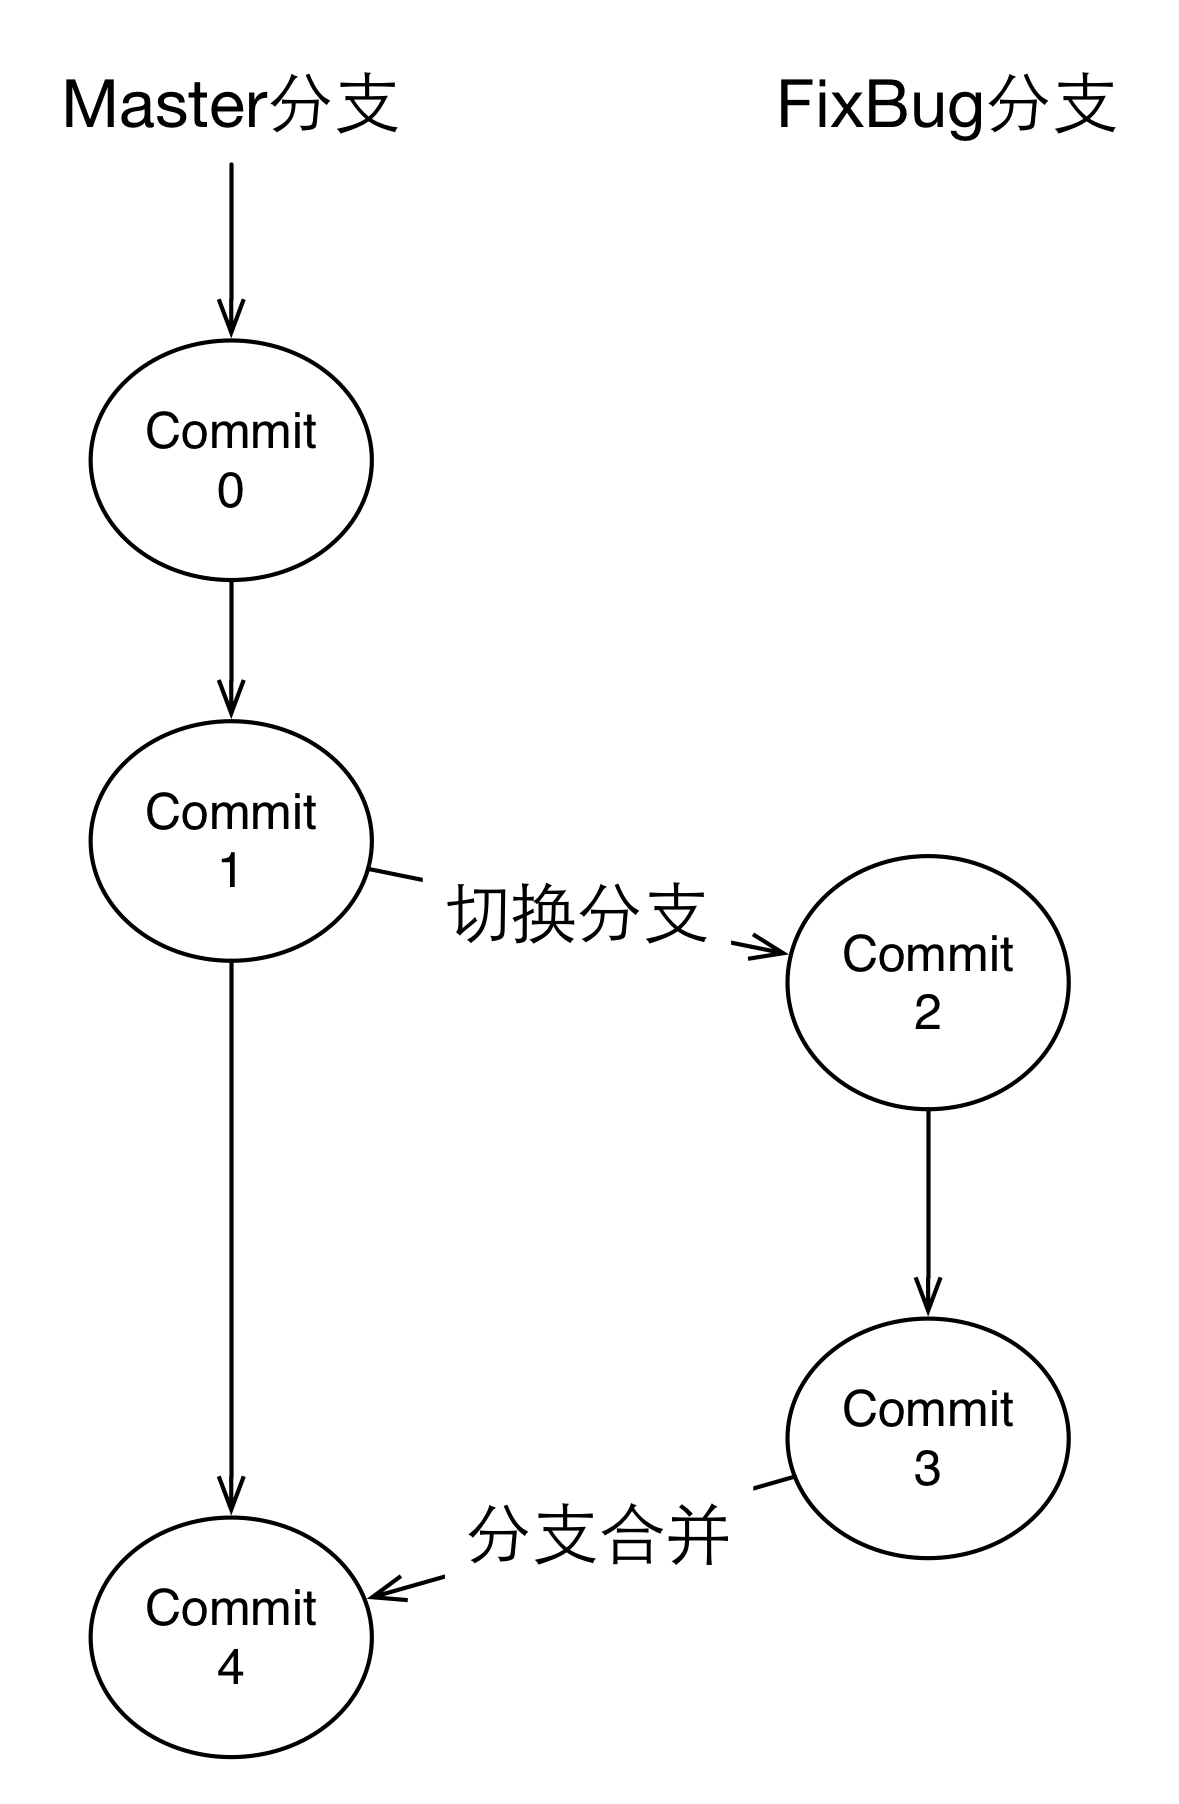
\includegraphics[width=.8\columnwidth]{chap03_git_branch}
	\caption {git分支切换与合并}	
	\label {git_branch}
\end{figure}


\subsection{补丁冲突}

为了确定补丁之间是否存在语义冲突,我们需要找到变更对于代码的语义影响。

\begin{definition}
	程序结构——指程序的基础语法结构,包括类、方法、基本块、语句等不同级别。
\end{definition}

\begin{definition}
	语义影响域(Sematic Impated Area)——在程序的某个限定范围中,直接或间接受到变更影响的程序结构集合。
\end{definition}

可见,语义影响域描述了变更对于程序中其他部分的影响。为了更清楚的理解,下面给出影响域的形式化定义。

\begin{definition}
	$impact: Patch \times Code \mapsto {Structure}$。$impact(p_m, v_k) = \{ \forall structure_j \subset Struct(v_k) \mid structure_j = im(sturcture_i), \exists change(structure_i) \subset p_m,structure_i,\subset Struct(v_k),v_k \subset Code,p_m \subset Pat(v_k), i,j,k,m \subset \mathbb{N} \}$。该函数用于描述补丁$p_m$对于其所应用的某个版本代码$v_k$的影响域。
\end{definition}

可以发现,为了解决问题\ref {compatible_formal},我们主要需要从代码中挖掘中两类信息:
\begin{enumerate}
	\item 代码的变更集合,即两个版本之间代码的差异性。
	\item 变更的影响集合,即变更集合对代码中其他哪些部分会造成影响。
\end{enumerate}

在有了这两类集合之后,我们就可以界定出软件变更在语义层面上对代码的语义影响域,我们可以将这整个过程称为语义影响域分析(Semantic Impacted Area Analysis)。

根据问题\ref {compatible_formal}中的描述,语义影响域分析可以划分为两个子过程:
\begin{enumerate}
	\item 程序间差异性分析:获取两个软件版本间的差异性,获得结构化的软件变更信息。该分析过程即为$diff(v_1,v_2)$函数的具体实现。
	\item 变更影响分析:分析软件变更对软件其他部分是否存在影响,并找到受影响的集合。该分析过程即为$impact(p_1,v_1)$函数的具体实现。
\end{enumerate}

我们可以将整个语义影响域分析过程定义为如下的函数:

\begin{definition}
	$s = ia(v_i,v_j) = impact(diff(v_i,v_j),v_i),i \subset \mathbb{N}, j \subset \mathbb{N}$
\end{definition}

通过语义影响域分析,我们就可以从代码中挖掘出所需要的变更影响信息,从而可以进行后续的分析工作。

事实上,可以将程序中受变更影响的部分划分为不同的粒度,从而获得不同程度的影响,我们考虑对面向对象的编程方法中的影响元素级别进行划分:

\begin{enumerate}
	\item 类:探讨变更对于其他类和对象的影响。对于面向对象的程序设计方法而言,这是最高级别的粒度。
	\item 方法:探讨变更对于其他方法的的影响。
	\item 基本块:探讨变更对于其他基本块的影响。
	\item 语句:探讨变更对于其他语句的影响。
\end{enumerate}

而所谓的影响范围也需要界定其粒度,不同层级的粒度显然会对语义影响域分析的精度产生影响。

\begin{enumerate}
	\item 类间:考虑变更的影响可能延伸到其他类、对象。
	\item 方法间:考虑变更的影响可能延伸到其他方法内部。
	\item 方法内部:考虑变更的影响只在本方法的内部延伸。
\end{enumerate}

在实际情况中,不同级别的影响范围均可分别采用不同的影响元素级别。

在有了软件变更的语义影响域之后,我们可以通过简单地比较两个补丁对代码的影响范围是否存在重叠来判定其是否发生了语义冲突。因此可以给出更详细的语义冲突的定义。

\begin{definition}
	\label {define_conflict}
	语义冲突(Semantic Confilict)——指两个补丁所对应的不同变更集合之间存在某两条互斥的变更。
	其中两条变更互斥指二者对同一行代码进行了修改,或者他们所修改了不同行代码,但其影响传播到了某行相同的代码。
\end{definition}

上述定义是对语义冲突的非形式化的描述,为了更清楚的理解,可以给出如下的形式化定义。

\begin{definition}
	\label {problem}
	如果$\exists c_m \subset p_i, \exists c_n \subset p_j$,其中$c_m = change(structure_m),c_n = change(structure_n)$, $structure_m \subset Struct(v_k), structure_n \subset Struct(v_k), v_k \subset Code$,并且$i,j,k,m,n \subset \mathbb{N}$。
	那么有$conflict(p_i,p_j) == true \iff (structure_m == structure_n) \lor (impact(p_i,v_k) \cap impact(p_j,v_k) \neq \varnothing)$,其中$p_i,p_j \subset Pat(v_k)$。
\end{definition}

可见,如果两个补丁对代码的影响域不存在重叠,那么他们两者之间自然是兼容的,因为他们不仅本身的变更互不干涉,并且他们所影响到的程序结构也互不干涉。在这样的情况下,补丁是可以成功应用到其他版本上的代码,并且可以完成补丁本身的目标的。

如果影响域发生了重叠,那么我们就可以认为补丁之间是不相容的,因为补丁所作的变更会对相同的程序结构产生影响。

实际上这样的影响是否能够兼容还需要人工的判定,因为在不同的情况下,他们可能是兼容的,也可能是不兼容的。而我们无法从代码中获取到足够的信息来进行这样的判定,需要人类对于变更的期望信息作为辅助。

我们可以将这个过程定义为如下类型的函数。可见,我们采用了$isCompatible(p_i,p_j)$函数来作为$conflict(p_i,p_j)$的具体实现。

\begin{definition}
	$isCompatible(p_i,p_j) : Patch \times Patch \mapsto Boolean$。其中$conflict(p_i,p_j) = isCompatible(p_i,p_j),i,j \subset \mathbb{N}$。
\end{definition}

显然,可以发现,问题\ref {compatible_formal}的核心在于:
\begin{itemize}
	\item 如何规约该问题?即$diff(v_i,v_j)$函数的实现。
	\item 如何计算影响域?即$impact(p_i,v_k)$函数的实现。
	\item 如何判定发生了冲突?即$conflict(p_i,p_j)$函数的实现。
\end{itemize}

\section{解决方案}

考虑前两节中所提到的应用场景和对问题的分析,我们可以给出一个通用的解决方案来解决整个兼容性问题的判定。

\subsection{整体架构}

可见,问题\ref{compatible}的解决主要需要采用对应的解决方法分别解决三个子问题,最后将再将其组合起来即可,是一个应用了分治法的解决方案。



可见,本文中给出了一个通用的补丁兼容性分析解决方案,可以通过更改相应的分析模块来提高解决方案的普遍适用性。解决方案中所涉及到的各个分析模块都可以更改其核心算法,采取不同的分析算法来完成相应的任务。

\subsection{补丁应用}

如问题\ref {patch_reversion}中所述,我们可以采用常见的版本控制工具提供的三路归并算法进行补丁的版本迁移工作。具体来讲,其流程可以简述如下:
\begin{enumerate}
	\item 采用git进行代码的版本管理,在主分支master中提交代码版本$v_1$。
	\item 切换到分支new,并提交新版本代码$v_2$。
	\item 将补丁$p_1$应用到版本$v_1$,获得旧版本应用补丁后的代码,即其版本为$v_3 = patch(p_1,v_1)$。
	\item 切换到分支patch,并提交代码版本$v_3$。
	\item 切换回分支new,将分支patch进行入分支new,获得新版本应用补丁后的代码,其版本为$v_4$。
	\item 解决分支合并中可能出现的冲突问题。
\end{enumerate}


其中,通过三路归并算法进行的合并工作中可能会出现冲突,这说明版本$v_2$和$v_3$之间存在语法冲突,即这两个版本在语法层面上不兼容。我们可以通过人工修改的方式进行修复,实现语法层面上的兼容性。

在解决冲突的过程中可以采用第三方的合并工具,利用现成工具的高效算法快速解决冲突。

\subsection{语义影响域分析}

如问题\ref {impacted_area}所述,我们需要进行语义影响域分析来获取两个补丁的影响范围,用于后续分析使用。

实际上,语义影响域分析主要分为两个分析过程,即程序间差异分析和变更影响分析,通过这两个分析的协作来完成整个语义影响范围的分析。

\subsubsection{程序差异性分析}

程序差异性分析主要用于分析两个不同版本的程序间的差异性,其结果即我们所需要的程序变更集合。近年来程序差异性分析方面有不少工作,实现了一些较为成熟的比较工具,我们可以使用这些工具来实现该分析过程。

在本文的组合架构中,程序差异性分析的主要任务是接受两个不同版本的源代码,并返回代码间的结构化差异信息。结构化的差异信息可以视为补丁的一种,只不过它具有比常见的采用Unix diff工具生成的$.patch$类型的补丁文件更丰富的信息,能够描述以程序语法结构的形式对软件变更进行描述。

该分析过程应该满足如下需要:
\begin{itemize}
	\item 输入为两个不同版本的代码。
	\item 输出为源代码间的软件变更集合。
	\item 每条变更描述语句或基本块级别的变更。
	\item 每条变更描述新旧程序结构的相关信息和其关联关系。
	\item 每条变更描述了其所属的作用域。
\end{itemize}

选择这样的分析结果类型是为了后续分析过程的方便,因为变更影响分析需要我们提供软件变更集合作为输入,而$.patch$类型的补丁文件只描述文本行的变更,不包含语法信息,我们无法从中提取出所需的语法层面的变更信息。

一种比较好的选择是采用AST差异性分析,因为抽象语法树中包括了足够多的语法结构信息。

该过程可以描述如图\ref {differ}。在实际过程中,Program Differ组件可以根据需要任意选择,只要其输入输出信息满足上述需求即可。图中所描述的软件变更集合可以定义如下:
\begin{definition}
	$ change\_set = \{ (old_i,new_i) \mid  old_i \subset Structure,new_i \subset Structure, i \subset \mathbb{N} \}$
\end{definition}

\begin{figure}[H]
	\centering
	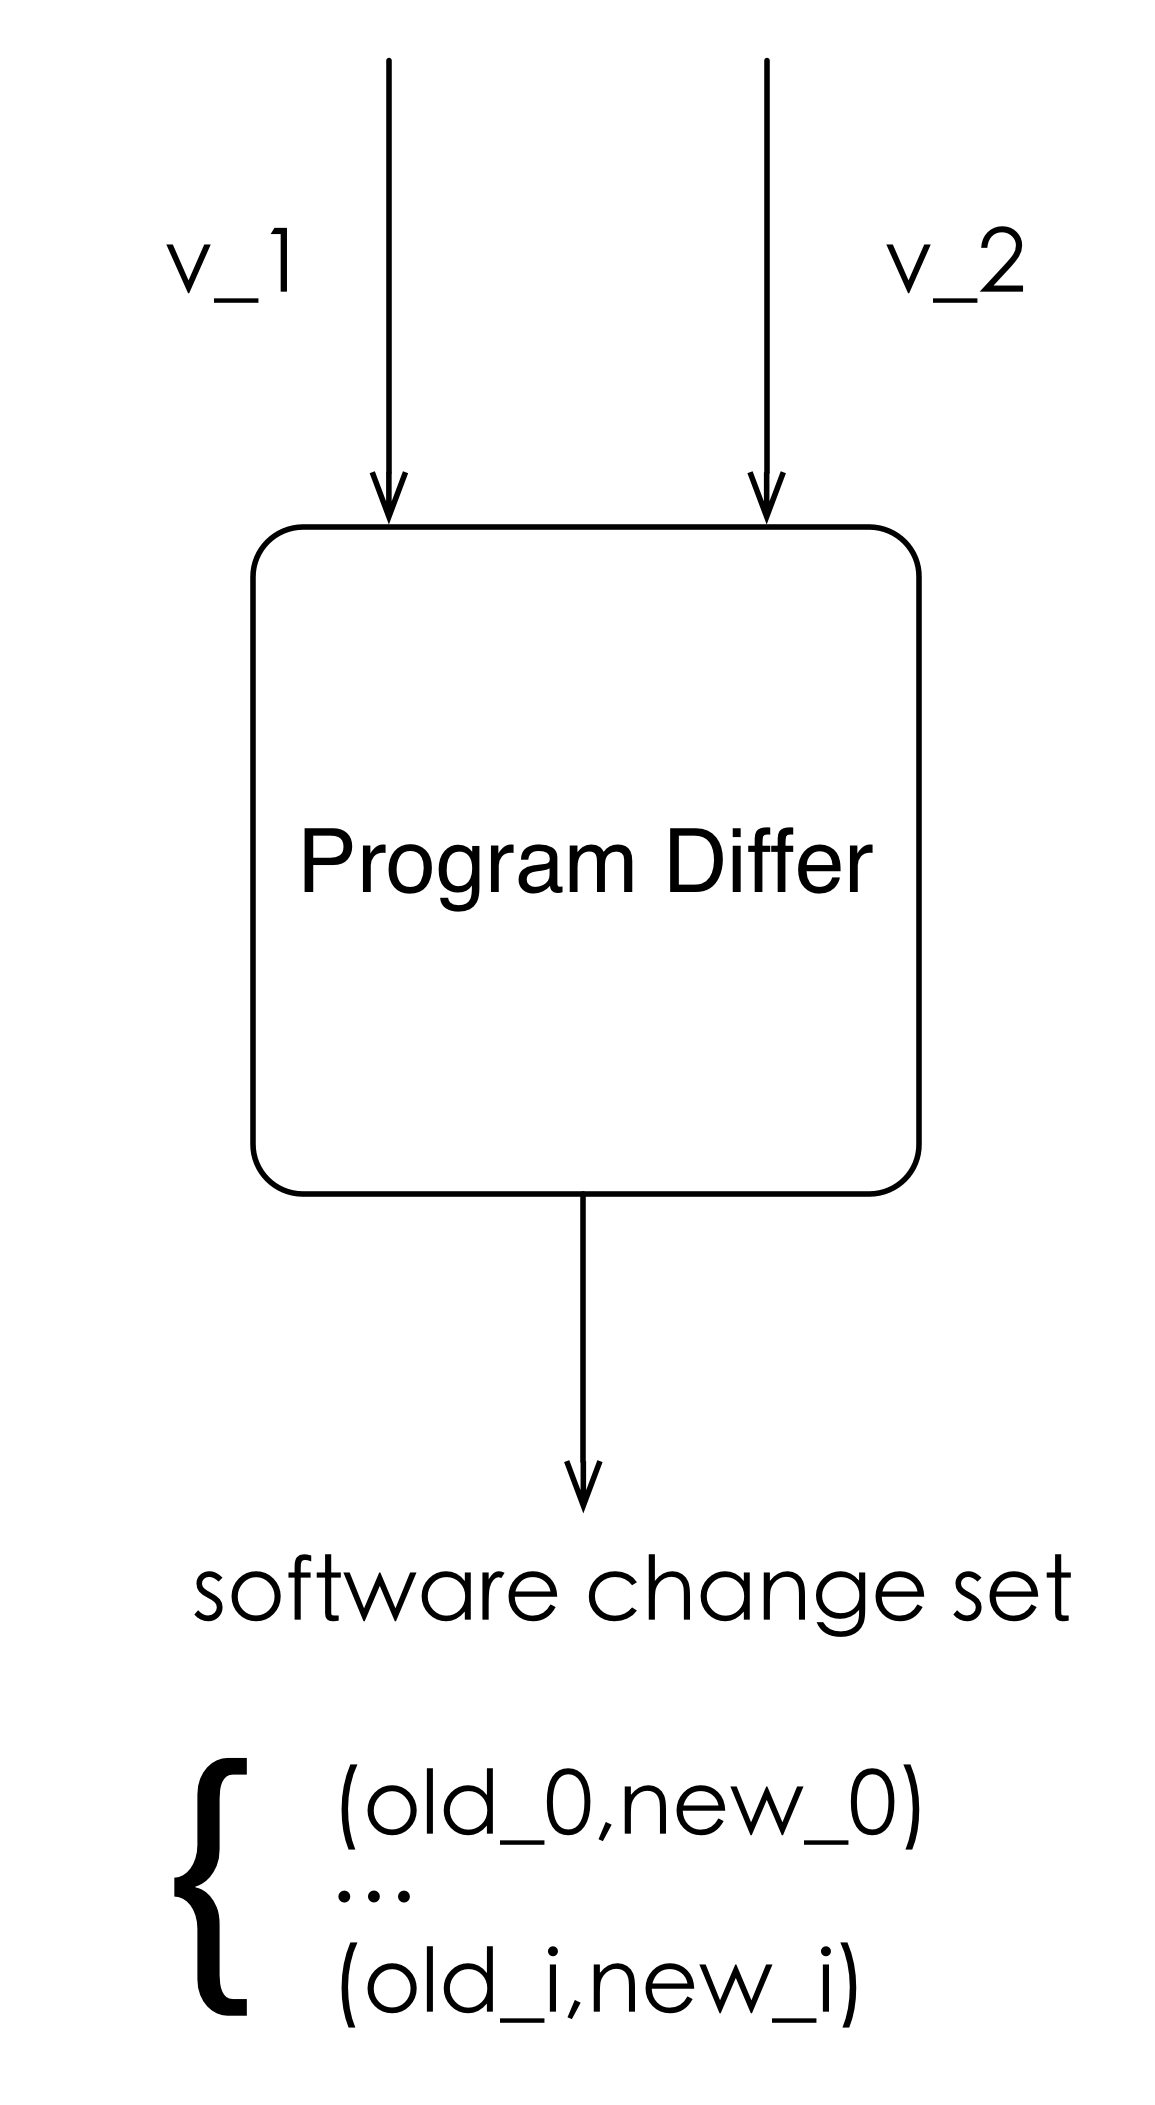
\includegraphics{chap03_differ}
	\caption {程序间差异分析}
	\label {differ}	
\end{figure}

\subsubsection{变更影响分析}

程序变更影响分析主要用于获取变更集合对其他程序结构的影响集合,该集合所包含的程序结构直接或间接地受到变更集合中的元素影响。近年来这方面比较成熟的工作也有不少,因而可以直接选择合适的变更影响分析算法作为该过分析过程的具体实现。

在本文的组合架构中,该分析过程应当接受两个不同版本代码间的变更集合作为输入,并输出变更集合所对应的影响集合,这也就是我们所需要的变更集合的语义影响范围。变更影响分析的过程可以通过控制流、数据流等信息分析出变更集合中每条变更对其他程序结构是否存在影响,并进行闭包计算即可。

本文对于该分析过程的要求如下:
\begin{itemize}
	\item 接受两个不同版本代码间的变更集合作为输入。
	\item 计算得到该变更集合所对应的影响集合。
	\item 计算过程中可以指定受影响的范围和元素类型。
	\item 影响集合中的元素按照其不同类型进行分类。
	\item 具有影响追踪系统,将计算影响集合的过程进行记录。方便后续的兼容性分析过程进行回溯。
\end{itemize}

其中影响追踪系统可以定义成如下类型的函数。该函数接受一个变更影响分析函数$ia(v_i,v_j)$,并返回对应的影响依赖关系集合。

\begin{definition}
	$impact\_track(ia(v_i,v_j))::(Code \rightarrow Code \rightarrow Impact Set) \rightarrow Impact Dependency$
\end{definition}


该分析过程如图\ref {impact_analyzer}所述,其中的impact analyzer组件可以任意选择某一能够满足上述要求的变更影响分析算法图中所描述的变更影响集合可以定义如下:
\begin{definition}
	$impact\_set = \{ (structure_i) \mid  structure_i \subset Structure, i \subset \mathbb{N}\}$
\end{definition}

\begin{figure}[H]
	\centering
	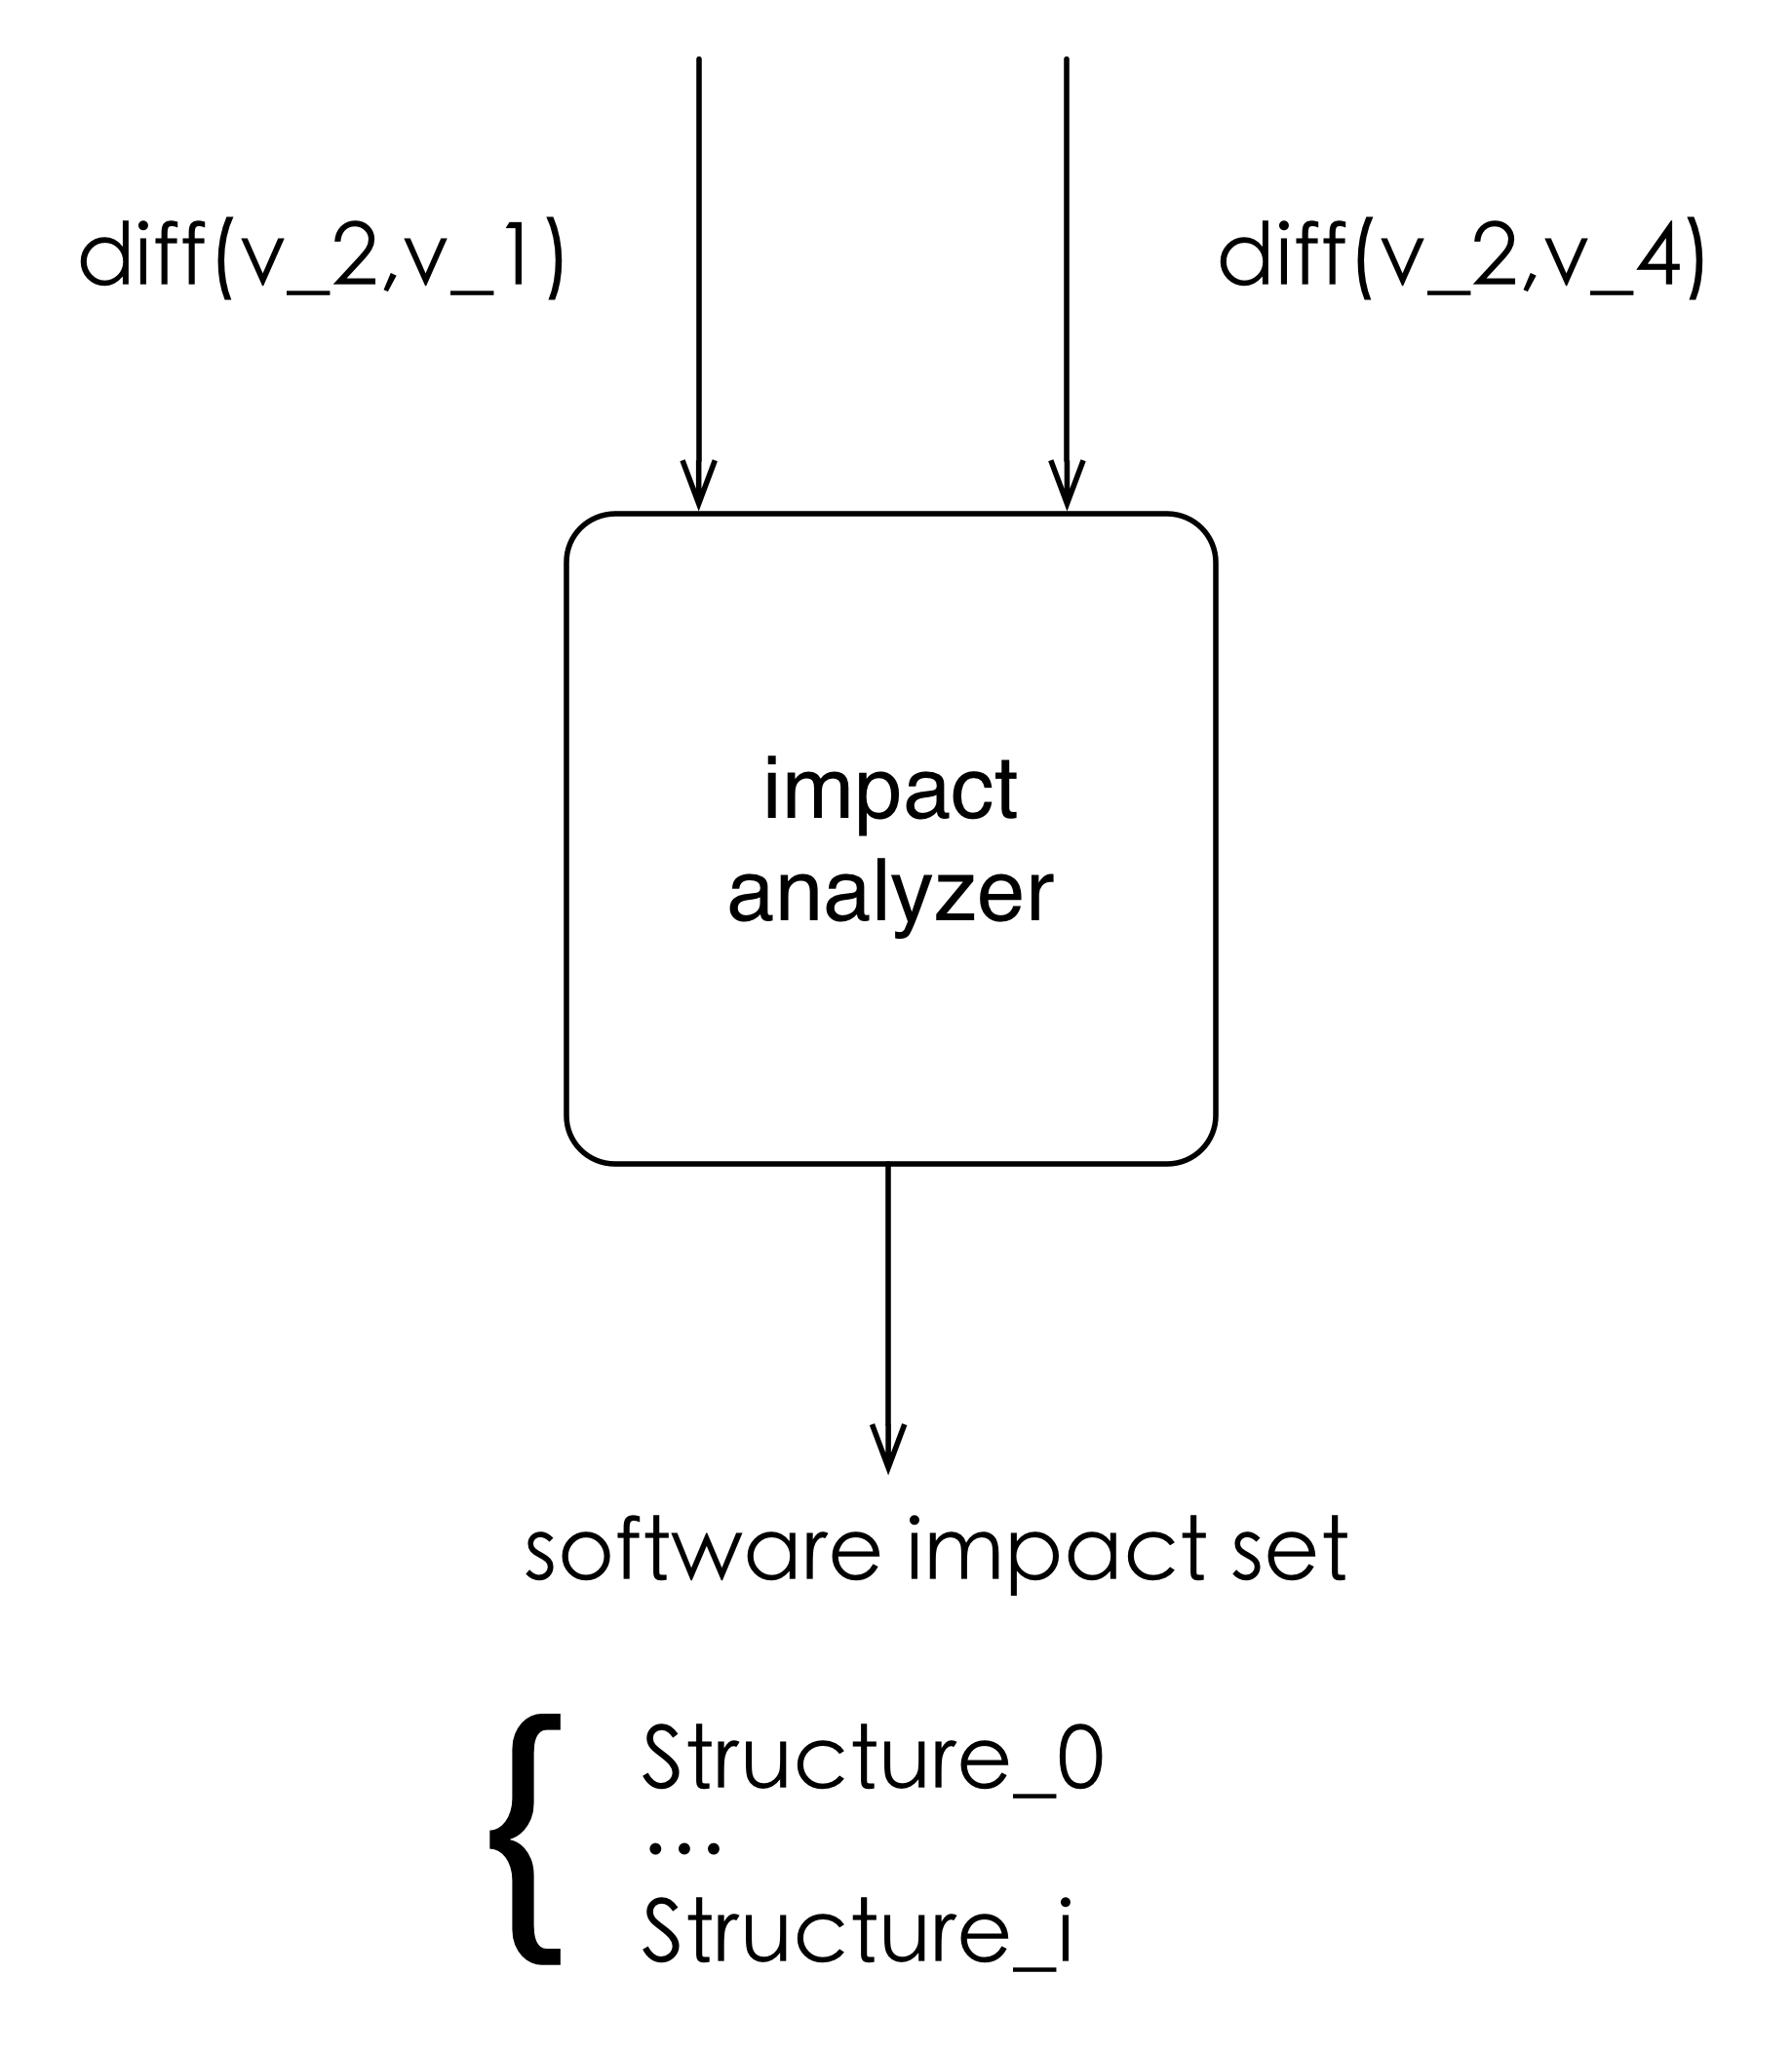
\includegraphics{chap03_impact}
	\caption {程序间差异分析}
	\label {impact_analyzer}	
\end{figure}

在完成了上述两项子分析过程后,我们就完成了整个语义影响域分析过程,并获得了两个不同版本代码的变更集合和对应的其语义影响范围。接下来就可以进行具体的兼容性分析工作。

\subsection{冲突分析}

在冲突分析中,我们将对比两个版本代码的影响范围,确定他们是否重叠,以此为依据判断其兼容性。

理论上来讲,这种简单比对即可发现两个版本间的兼容性问题,因为一旦发生重叠,那么重叠的代码部分显然是会发生兼容性问题的。然而在实际情况中,受限于工具的精度,我们往往不能达到理论上的准确度,而可能会发生误报(false positive)等情况。

显然,如果重叠不存在,则兼容性是可以得到满足的。而对于如何界定重叠部分的兼容性,则需要人工分析的介入,因为这部分代码的兼容性与补丁的功能目标密切相关,而我们无法从代码中获取到这种信息,因而只有依靠外界来提供,并以此为依据进行详细分析过程,界定这部分代码是否真的存在冲突。

在进行人工分析的过程中,我们不仅需要知道哪部分代码出现了重叠现象,而且还需要知道是哪些变更影响到了这部分代码,因而我们需要引入影响追踪系统来记录变更影响分析过程的轨迹。影响追踪系统可以记录下变更影响分析过程中的每一步,从而获取到程序结构间的影响关系链,事后通过回溯即可追踪到具体的软件变更可见,本过程中主要需要影响追踪系统的回溯模块的支持。

可以看得出来,由于使用了更严格的冲突定义,我们的方法会造成一定的过高估计的结果。

该分析过程可以参考算法\ref {algo_compatible}。

\begin{algorithm}
	\caption{冲突分析}
	\label{algo_compatible}
	\begin{algorithmic}[1]
		\REQUIRE $s_1=ia(v_2,v_1)$,$s_2=ia(v_2,v_4)$\\
				 \quad \quad $t_1=impact\_track(ia(v_2,v_1))$, $t_2=impact\_track(ia(v_2,v_4))$
		\ENSURE $isCompatible(diff(v_2,v_1), diff(v_2,v_4))$
		\IF{$s_1 = \varnothing \lor s_2 = \varnothing$}
			\STATE $result \gets True$
		\ELSE
			\STATE $s \gets s_1 \cap s_2$
			\IF{$s = \varnothing$}
				\STATE $result \gets True$
			\ELSE				
				\STATE $result \gets Manual\_analysis(s_1, s_2, t_1, t_2)$
			\ENDIF 
		\ENDIF
		\RETURN $result$
	\end{algorithmic}
\end{algorithm}

整个分析过程的架构如图\ref {isCompatible}所示。

\begin{figure}[H]
	\centering
	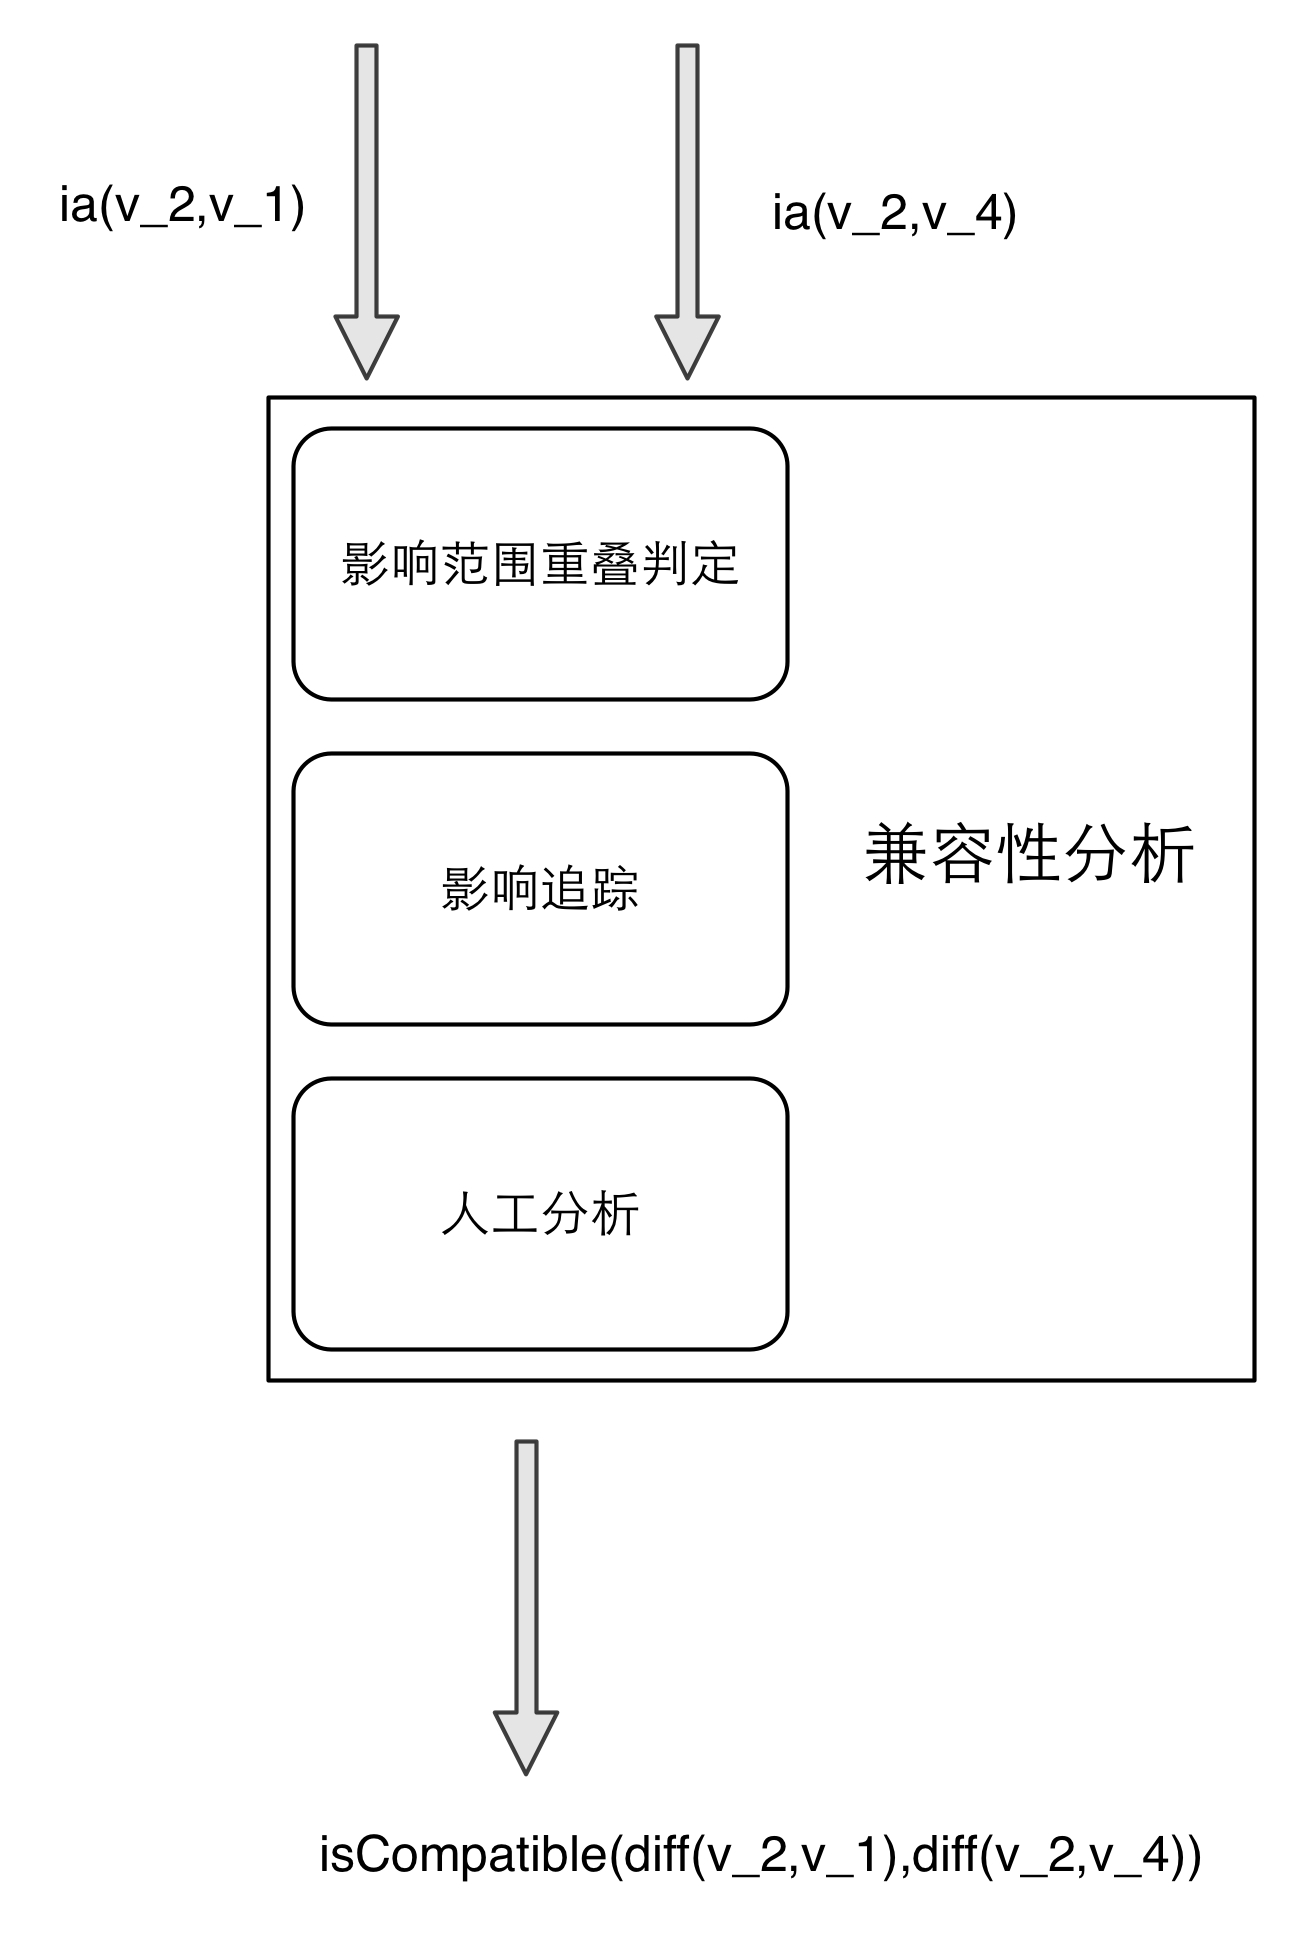
\includegraphics{chap03_isCompatible}
	\caption {兼容性分析}
	\label {isCompatible}	
\end{figure}


\section{本章小结}